% =====================================================================
%  polymirror: Mirror-trading on Polymarket, a leakage-controlled
%  backtest and a live forward test.
%
%  Overleaf-ready. Compiles with pdfLaTeX (no external images required;
%  the edge-decay figure is drawn with pgfplots from embedded data).
%  Recommended Overleaf setting: TeX Live 2021+ / pdfLaTeX.
% =====================================================================
\documentclass[11pt]{article}

\usepackage[utf8]{inputenc}
\usepackage[T1]{fontenc}
\usepackage[margin=1in]{geometry}
\usepackage{amsmath,amssymb}
\usepackage{booktabs}
\usepackage{array}
\usepackage{textcomp}
\usepackage{graphicx}
\usepackage{subcaption}
\usepackage{caption}
\usepackage{xcolor}
\usepackage[hidelinks]{hyperref}
\graphicspath{{figs/}}

\title{\textbf{Does Copying Skilled Wallets Beat Buying the Favorite?}\\[2pt]
\large Evidence from a Leakage-Controlled Backtest and a Live Forward Test
on Polymarket}

\author{polymirror project\\
\small Read-only study of prediction-market mirror-trading\\
\small Run dated 2026-06-07/09; all code, parameters, and seeds in the accompanying repository}
\date{}

\begin{document}
\maketitle

\begin{abstract}
\noindent
We ask whether a strategy that \emph{mirrors} the entries of high-quality Polymarket
wallets can outperform a \emph{buy-the-favorite} benchmark, after costs, over short
holding horizons. We attack the question two independent ways. \textbf{Study 1} is a
strictly leakage-controlled \emph{historical} test: every sufficiently active wallet is
scored with the Brier proper score over resolved binary markets and subjected to a
skill-vs-luck filter (a Bernoulli-price null, $10{,}000$-draw bootstrap, Benjamini--Hochberg
FDR control). \textbf{Of 151 wallets tested, zero survive} the filter at any activity
floor, even before multiple-testing correction, and with a minimum $p$-value of $0.305$.
\textbf{Study 2} is a \emph{live forward} test over a single $48$\,h window: we
abandon the (empty) skill-filtered watchlist and instead mirror the top-10 active wallets
from the Polymarket profit leaderboard, capturing $50{,}642$ real trades across $753$ markets
and reconstructing hour-by-hour returns from the CLOB price-history API. The forward mirror
\emph{under}-performs the favorite at short horizons: clustered by market (the correct unit,
$n\approx214$--$1{,}763$) the gross edge is $-5.9\%$ to $-8.7\%$ at every horizon from $1$ to
$12$\,h, with the $95\%$ bootstrap CI excluding zero throughout and $p$ as low as $0.003$: a
\textbf{statistically significant loss to mirroring}, the study's only significant result, and
signed in the wrong direction for copy-trading. Clustered by wallet the same estimates are
insignificant, because the six active wallets disagree in sign; horizons beyond ${\sim}13$\,h
swing in sign with cohort composition and settle nothing. \emph{Both} legs lose money in
absolute, gross-of-cost terms. Two methods, one conclusion: \textbf{we find no exploitable
mirror-trading edge}; if anything, mirroring reliably pays the post-information price. A
defensible null is the result.
\end{abstract}

% ---------------------------------------------------------------------
\section{Research question and design philosophy}
% ---------------------------------------------------------------------
\noindent
\textit{To what extent can a strategy that mirrors wallets identified as high-quality
outperform buy-and-hold-the-favorite over short holding horizons, after costs?}

\medskip
The unit of analysis is the on-chain wallet (\texttt{proxyWallet}); a wallet is not a person.
The evaluation standard is empirical honesty, not profit: a defensible null is a success, and a
profitable-looking result resting on a hidden bias is a failure. The headline object is an
\emph{edge-decay curve} (edge $=$ (mirror $-$ benchmark) return as a function of holding
horizon $N$), not a single number. Eight design rules govern the work
(Table~\ref{tab:rules}); each, if violated, invalidates a result. Study~2 deliberately and
explicitly relaxes rule R2 (\S\ref{sec:selection}) and is therefore labeled exploratory; that
deviation was forced by Study~1's empty survivor set and is itself a finding.

\begin{table}[h]
\centering
\caption{Design rules. Violating any one invalidates the affected result.}
\label{tab:rules}
\small
\begin{tabular}{@{}cp{13.2cm}@{}}
\toprule
\textbf{R0} & Historical / read-only. No live trade, no private key, no funded wallet; every API call is a GET. \\
\textbf{R1} & Strict temporal train/test split; selection statistics use training-window trades only. \\
\textbf{R2} & Ex-ante, machine-evaluable accuracy $=$ a proper score (Brier / log loss), never raw PnL, leaderboard, or reputation. \\
\textbf{R3} & Skill-vs-luck filter: a wallet is eligible only if it beats a luck null, not merely ranks high. \\
\textbf{R4} & ``Favorite'' defined at entry (mid $>0.5$ at the entry timestamp), never with hindsight. \\
\textbf{R5} & Strategy and benchmark identical except which side is bought: same trigger, exit rule, costs, spread. \\
\textbf{R6} & Spread is a swappable, labeled parameter; every headline reported under all three presets; a result surviving only the optimistic preset is \emph{not} a result. \\
\textbf{R7} & Wallet $\neq$ person (stated limitation). \\
\textbf{R8} & Reproducibility: one \texttt{config.py} drives all parameters; every stochastic step is explicitly seeded. \\
\bottomrule
\end{tabular}
\end{table}

% ---------------------------------------------------------------------
\section{Data and the binding constraints}
% ---------------------------------------------------------------------
Three public, no-authentication Polymarket APIs are used. \textbf{Gamma}
(\texttt{gamma-api.polymarket.com}) supplies markets and ground-truth resolution: a binary
market is resolved iff \texttt{closed==true} and \texttt{outcomePrices}~$\in
\{[\,1,0\,],[\,0,1\,]\}$, the winning index is the position of the ``1'', and settlement time
is \texttt{closedTime}. The \textbf{Data API} (\texttt{data-api.polymarket.com}) supplies
per-wallet and per-market trade records; \texttt{/trades} ignores \texttt{start}/\texttt{end}
and caps at the $\sim$4{,}000 most-recent records per market, whereas \texttt{/activity}
honors \texttt{start}/\texttt{end} (used for forward capture). The \textbf{CLOB}
(\texttt{clob.polymarket.com}) supplies \texttt{/midpoint}, \texttt{/spread}, and
\texttt{/prices-history}.

\paragraph{A methodological correction.} Earlier project notes assumed the order book is
destroyed on resolution, forcing historical marks to be rebuilt from trade prints. We find
this is only true for long-pruned markets: \texttt{/prices-history} returns a \emph{one-minute}
mid series that \emph{persists for days} after resolution (verified: a market resolved
$\sim$6 days earlier still returned its full series; a $1.5$-year-old market was pruned to
empty). This is what makes a low-frequency, on-demand forward design feasible: exit marks are
reconstructed retrospectively, so the collector needs network access only at capture and
analysis time, not continuously at each horizon.

% ---------------------------------------------------------------------
\section{Study 1: Historical skill-vs-luck filter}
% ---------------------------------------------------------------------
\subsection{Method}
For every wallet with at least $k$ resolved BUY entries (activity floors $k\in\{8,10,15\}$),
we collapse all fills in a market to \emph{one position per (wallet, market, outcome)}: a
size-weighted mean entry price $p$ and a single realized outcome $y\in\{0,1\}$. This collapse
is essential: a wallet placing $71$ fills in one market has made \emph{one} correlated bet,
not $71$, and treating them as independent inflates naive $t$-statistics several-fold. Each
wallet receives a Brier score $\tfrac1n\sum_i (p_i-y_i)^2$. We then test it against a luck null:
holding entry prices $p_i$ fixed, redraw outcomes $y_i^\ast\sim\mathrm{Bernoulli}(p_i)$
$10{,}000$ times and recompute the score; this yields the distribution of a wallet with \emph{no skill
beyond the market price}. The empirical $p$-value is Laplace-smoothed,
$\bigl(\#\{\text{null}\le\text{observed}\}+1\bigr)/(n_{\text{boot}}+1)$, with each wallet's RNG
seeded from $\texttt{seed}\oplus\mathrm{blake2b}(\text{wallet})$. Benjamini--Hochberg FDR
control is applied across wallets; we report both raw and FDR survivors. The Bernoulli-price
null is deliberately strict: it subsumes the favorite-buyer fallacy, since buying at $0.84$ and
winning $84\%$ of the time is exactly what the null does, and earns no significance.

\subsection{Results: zero survivors}
The candidate pool, built from $60$ high-volume resolved binary markets (2026 settlement),
yielded \textbf{85{,}184 positions across 67{,}489 wallets}. Applying the activity floors gives
Table~\ref{tab:survivors}: \textbf{no wallet survives at any floor}, raw or FDR-corrected.

\begin{table}[h]
\centering
\caption{Skill-vs-luck filter outcomes. Under pure chance, ${\sim}7$--$8$ raw survivors would
be expected at floor $k=8$; observing zero is a strong null.}
\label{tab:survivors}
\small
\begin{tabular}{@{}lccc@{}}
\toprule
Activity floor (positions) & Wallets tested & Raw survivors ($p<0.05$) & FDR survivors \\
\midrule
$\ge 8$  & 151 & \textbf{0} & \textbf{0} \\
$\ge 10$ & 79  & \textbf{0} & \textbf{0} \\
$\ge 15$ & 27  & \textbf{0} & \textbf{0} \\
\bottomrule
\end{tabular}
\end{table}

The result is not marginal. Across the $151$ tested wallets the \textbf{minimum $p$-value is
$0.305$}; the $p$-value distribution piles up at the top of the unit interval
(Table~\ref{tab:pdist}), with \emph{none} below $0.30$. The mean null margin (observed $-$ null
Brier) is $+0.0024$ and $17\%$ of wallets score \emph{worse} than their own price-null: the
population is not merely unskilled but, on average, at or slightly below the price-implied
benchmark. Table~\ref{tab:best} lists the fifteen best-ranked wallets for completeness; even the
strongest is indistinguishable from luck.

\begin{table}[h]
\centering
\caption{$p$-value distribution across the 151 tested wallets (floor $k=8$).}
\label{tab:pdist}
\small
\begin{tabular}{@{}lcccccccccc@{}}
\toprule
Decile & $[.0,.1)$ & $[.1,.2)$ & $[.2,.3)$ & $[.3,.4)$ & $[.4,.5)$ & $[.5,.6)$ & $[.6,.7)$ & $[.7,.8)$ & $[.8,.9)$ & $[.9,1.0)$ \\
\midrule
Count & 0 & 0 & 0 & 3 & 0 & 1 & 1 & 2 & 18 & 126 \\
\bottomrule
\end{tabular}
\end{table}

\begin{figure}[h]
\centering
\begin{subfigure}{0.62\textwidth}
  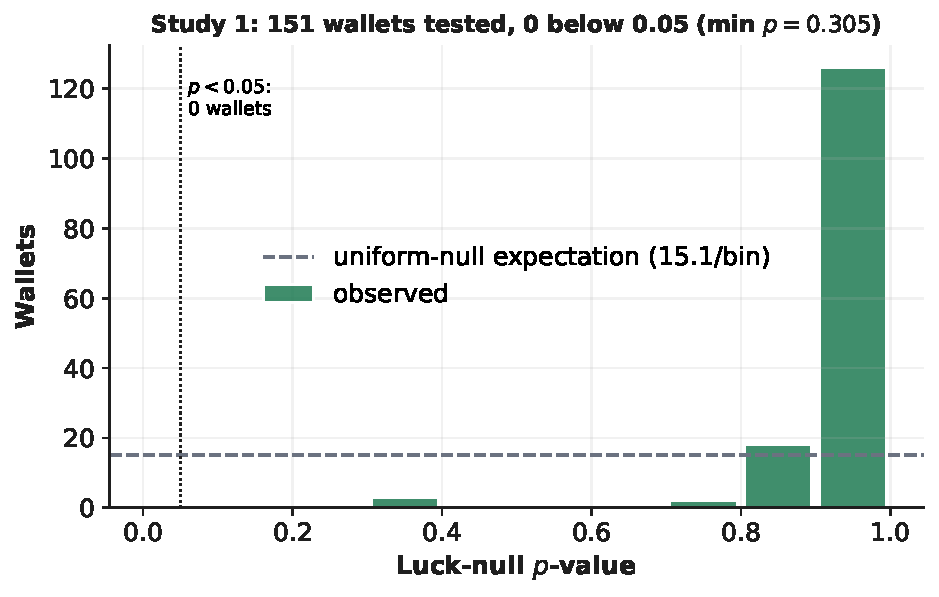
\includegraphics[width=\linewidth]{fig_s1_pvalue_dist.pdf}
  \caption{$p$-value distribution vs.\ the uniform-null expectation.}
\end{subfigure}\hfill
\begin{subfigure}{0.36\textwidth}
  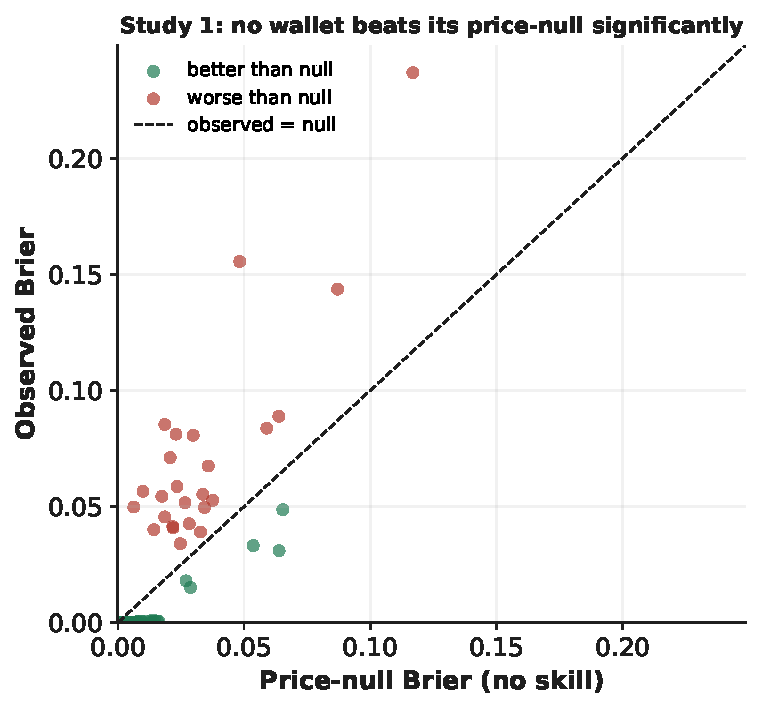
\includegraphics[width=\linewidth]{fig_s1_brier_scatter.pdf}
  \caption{Observed vs.\ price-null Brier.}
\end{subfigure}
\caption{Study 1 evidence. Left: the $p$-value mass sits far above the $\alpha=0.05$ line, with
none below $0.30$, against the flat distribution expected if even a few wallets were skilled.
Right: most wallets lie on or above the $45^\circ$ line (observed Brier $\ge$ price-null Brier),
i.e.\ no better than no-skill pricing. No wallet is significant.}
\label{fig:s1}
\end{figure}

\begin{figure}[h]
\centering
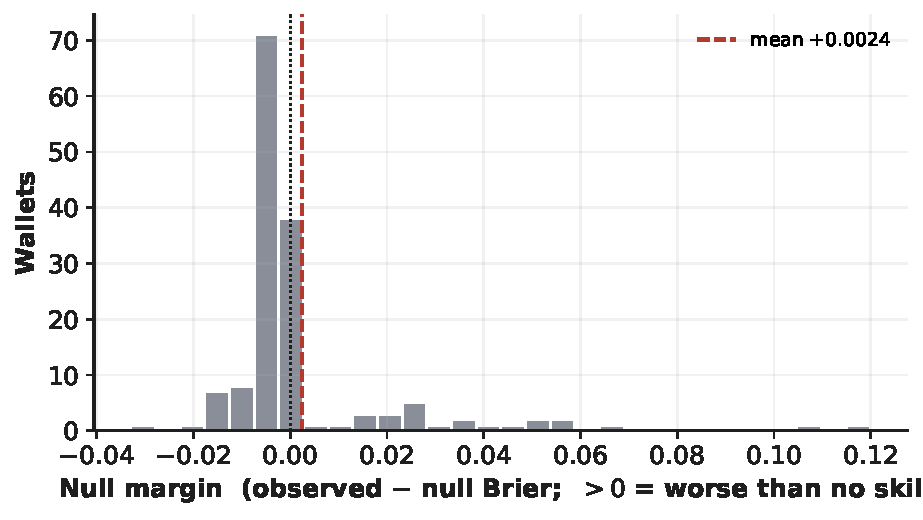
\includegraphics[width=0.72\textwidth]{fig_s1_null_margin.pdf}
\caption{Study 1: distribution of the null margin (observed $-$ price-null Brier) across the 151
tested wallets. The mass is centered near zero with a slightly positive mean ($+0.0024$); $17\%$
of wallets score \emph{worse} than their own price-null. The population shows no calibration skill
beyond the market price.}
\label{fig:s1margin}
\end{figure}

\begin{table}[h]
\centering
\caption{Fifteen best-ranked wallets by luck-null $p$-value (floor $k=8$). \texttt{null} is the
mean Brier of the Bernoulli-price null; \texttt{margin} $=$ observed $-$ null ($<0$ is better
than the null). None reaches significance.}
\label{tab:best}
\small
\begin{tabular}{@{}lrrrrrr@{}}
\toprule
Wallet (truncated) & $n_{\text{pos}}$ & $n_{\text{mkt}}$ & Brier & null & margin & $p$ \\
\midrule
0x3d03\dots249d52 &  8 &  8 & 0.0487 & 0.0654 & $-0.0167$ & 0.305 \\
0xed45\dots970d29 &  9 &  8 & 0.0332 & 0.0537 & $-0.0205$ & 0.367 \\
0x9cdd\dots3d3e97 &  8 &  8 & 0.0310 & 0.0639 & $-0.0329$ & 0.395 \\
0xc6dd\dots913987 & 11 & 11 & 0.0180 & 0.0270 & $-0.0090$ & 0.527 \\
0x9aeb\dots5b2729 &  9 &  9 & 0.0152 & 0.0288 & $-0.0136$ & 0.615 \\
0x7c3d\dots1e5c6b & 18 & 17 & 0.0391 & 0.0328 & $+0.0063$ & 0.738 \\
0x5b63\dots9c911a4 & 35 & 28 & 0.0004 & 0.0077 & $-0.0073$ & 0.749 \\
0x24c8\dots2e823e1 & 29 & 21 & 0.0002 & 0.0071 & $-0.0069$ & 0.809 \\
0xafaa\dots2dff0e4 & 10 &  7 & 0.0527 & 0.0376 & $+0.0151$ & 0.833 \\
0x12d6\dots2cf2a8 & 15 & 13 & 0.0340 & 0.0248 & $+0.0092$ & 0.838 \\
0x5a21\dots7809318 & 10 &  8 & 0.0007 & 0.0162 & $-0.0155$ & 0.843 \\
0x72a2\dots428e7b65 & 15 & 15 & 0.0414 & 0.0218 & $+0.0196$ & 0.846 \\
0x8f7a\dots cdbdb40 & 15 & 13 & 0.0007 & 0.0092 & $-0.0085$ & 0.856 \\
0xe807\dots2ee4d35 &  8 &  7 & 0.0838 & 0.0590 & $+0.0247$ & 0.859 \\
0xb665\dots1ee2eed24 & 19 & 17 & 0.0002 & 0.0077 & $-0.0075$ & 0.860 \\
\bottomrule
\end{tabular}
\end{table}

\paragraph{Interpretation.} Under the project's own pre-registered eligibility rule (R3) the
historical data admit \emph{no} wallet worth mirroring, consistent with short-horizon
informational efficiency of these markets and with the literature finding that apparent skill
in large trader populations is overwhelmingly luck once multiple testing is controlled.

% ---------------------------------------------------------------------
\section{Study 2: Live forward mirror experiment}
% ---------------------------------------------------------------------
\subsection{Selection: an explicit R2 deviation}\label{sec:selection}
Because Study~1 left an empty watchlist, a confirmatory forward test of ``skilled'' wallets was
impossible. We therefore ran an \emph{exploratory} forward test using a different,
openly-labeled rule: the top-10 wallets by 30-day profit on the Polymarket leaderboard
(\texttt{lb-api.polymarket.com/profit?window=30d}), each verified currently active via a live
\texttt{/activity} check. This \textbf{violates R2} (selection by realized PnL/reputation) and is
reported as hypothesis-generating. The question it answers is narrower and more practical:
\emph{if a retail user naively copies whoever is winning right now, do they beat buying the
favorite?}

\subsection{Capture and mark-to-market}
Over a single window (2026-06-07 20:04 UTC $\to$ 2026-06-09 20:04 UTC; nominally a 6-hour
evening session extended to 48\,h), an on-demand puller recorded \emph{every} trade (BUY and
SELL) the ten wallets made in live binary markets. Each trade is normalized to an equivalent
opening \emph{long} (a SELL of token $k$ at $p$ is copied as a long of the complement at $1-p$):
we copy the \emph{action}, acknowledging a SELL may be profit-taking rather than a fresh view.
For each position we reconstruct, from \texttt{/prices-history}, the mid of both outcome tokens
at entry and at each elapsed hour $N$; horizons past resolution settle to $0/1$ (Gamma). The
\textbf{strategy leg} is the copied long; the \textbf{benchmark leg} is the favorite-at-entry
token; the two share entry timing and exit rule and differ only in side (R5). Returns are
computed gross, then (as in Study~1) collapsed to one position per (wallet, market, side)
before aggregation; inference is reported under both wallet-level and market-cell clustering.
All $999{,}012$ marks were reconstructed with \emph{zero missing} ($263{,}242$ from live
history, $735{,}770$ from settlement); no horizon was silently filled.

\subsection{Sample}
Table~\ref{tab:sample} summarizes the capture. The effective wallet count remains the dominant
limitation: four of ten leaderboard wallets never traded in the window, and inference rests on
\textbf{6 active wallets}, three of which supply $93\%$ of positions (Table~\ref{tab:wallets}).
The copied side coincided with the favorite in $39.8\%$ of positions, a genuine mix rather than
pure favorite-buying.

\begin{table}[h]
\centering
\caption{Forward capture summary.}
\label{tab:sample}
\small
\begin{tabular}{@{}lr@{}}
\toprule
Window & 2026-06-07 20:04 $\to$ 2026-06-09 20:04 UTC \\
Positions captured & 50{,}642 (49{,}945 BUY / 697 SELL) \\
Distinct markets & 753 (mostly same-day live sports) \\
Resolved positions by close & 37{,}806 \\
Marks reconstructed & 999{,}012 (history 263{,}242 / settle 735{,}770; missing 0) \\
Copied side $=$ favorite & 20{,}154 / 50{,}642 \;($39.8\%$) \\
Entry price (min / median / max) & 0.001 / 0.430 / 0.980 \\
Fills per market (max / median / mean) & 3{,}834 / 16 / 67.3 \\
\bottomrule
\end{tabular}
\end{table}

\begin{table}[h]
\centering
\caption{Per-wallet activity. Four of ten leaderboard wallets placed zero trades in the window.}
\label{tab:wallets}
\small
\begin{tabular}{@{}lr@{}}
\toprule
Wallet & Positions \\
\midrule
ferrariChampions2026  & 18{,}764 \\
Countryside           & 15{,}274 \\
HomeRunHazard         & 13{,}113 \\
PalestineChicken      & 1{,}940 \\
afghj2421             & 1{,}467 \\
jalenbrunson-official & 84 \\
(four others)         & 0 \\
\bottomrule
\end{tabular}
\end{table}

\subsection{Results: a significant short-horizon under-performance}
Table~\ref{tab:edge} reports the edge-decay curve at selected horizons (all $47$ populated
horizons are tabulated in Appendix~\ref{app:fulledge}), and Figure~\ref{fig:edge} plots the
two legs. Three observations decide the interpretation.

\begin{table}[h]
\centering
\caption{Forward edge-decay curve at selected horizons (gross of spread; one position per
wallet/market/side). ``By wallet'' clusters across the active wallets ($n{=}6$ for $N\le18$,
$5$ at $19$\,h, $4$ for $N\ge20$); ``by market'' clusters across the independent market-cells
($n$ shown). $95\%$ CIs and two-sided $p$-values are from a seeded $10{,}000$-resample
bootstrap. Appendix~\ref{app:fulledge} reports all horizons.}
\label{tab:edge}
\small
\setlength{\tabcolsep}{4pt}
\begin{tabular}{@{}rrr rcc rcc@{}}
\toprule
& \multicolumn{2}{c}{Returns (gross)} & \multicolumn{3}{c}{By wallet} & \multicolumn{3}{c}{By market} \\
\cmidrule(lr){2-3}\cmidrule(lr){4-6}\cmidrule(lr){7-9}
$N$(h) & Mirror & Favorite & Edge & 95\% CI & $p$ & Edge & 95\% CI ($n$) & $p$ \\
\midrule
1 & $-0.091$ & $+0.005$ & $-0.096$ & $[-0.274,+0.019]$ & 0.213 & $-0.059$ & $[-0.105,-0.012]$ (1{,}763) & 0.013 \\
2 & $-0.002$ & $+0.072$ & $-0.074$ & $[-0.281,+0.100]$ & 0.448 & $-0.080$ & $[-0.132,-0.026]$ (1{,}744) & 0.003 \\
3 & $-0.097$ & $-0.064$ & $-0.033$ & $[-0.279,+0.231]$ & 0.714 & $-0.076$ & $[-0.133,-0.019]$ (1{,}696) & 0.011 \\
4 & $-0.122$ & $-0.090$ & $-0.032$ & $[-0.283,+0.249]$ & 0.735 & $-0.077$ & $[-0.135,-0.020]$ (1{,}659) & 0.010 \\
6 & $-0.126$ & $-0.092$ & $-0.035$ & $[-0.295,+0.269]$ & 0.759 & $-0.081$ & $[-0.142,-0.019]$ (1{,}550) & 0.011 \\
8 & $-0.127$ & $-0.094$ & $-0.033$ & $[-0.293,+0.272]$ & 0.767 & $-0.080$ & $[-0.142,-0.016]$ (1{,}436) & 0.015 \\
12 & $-0.126$ & $-0.097$ & $-0.029$ & $[-0.291,+0.275]$ & 0.776 & $-0.069$ & $[-0.136,-0.000]$ (1{,}240) & 0.050 \\
16 & $-0.124$ & $-0.096$ & $-0.029$ & $[-0.288,+0.276]$ & 0.776 & $-0.071$ & $[-0.147,+0.005]$ (1{,}129) & 0.067 \\
24 & $+0.131$ & $-0.039$ & $+0.170$ & $[-0.078,+0.646]$ & 0.626 & $-0.062$ & $[-0.158,+0.038]$ (737) & 0.211 \\
36 & $-0.021$ & $+0.018$ & $-0.038$ & $[-0.075,-0.009]$ & 0.006 & $-0.037$ & $[-0.171,+0.100]$ (398) & 0.585 \\
47 & $-0.154$ & $-0.275$ & $+0.122$ & $[+0.046,+0.190]$ & 0.006 & $+0.187$ & $[-0.015,+0.400]$ (214) & 0.074 \\
\bottomrule
\end{tabular}
\end{table}

\begin{figure}[h]
\centering
\begin{subfigure}{0.49\textwidth}
  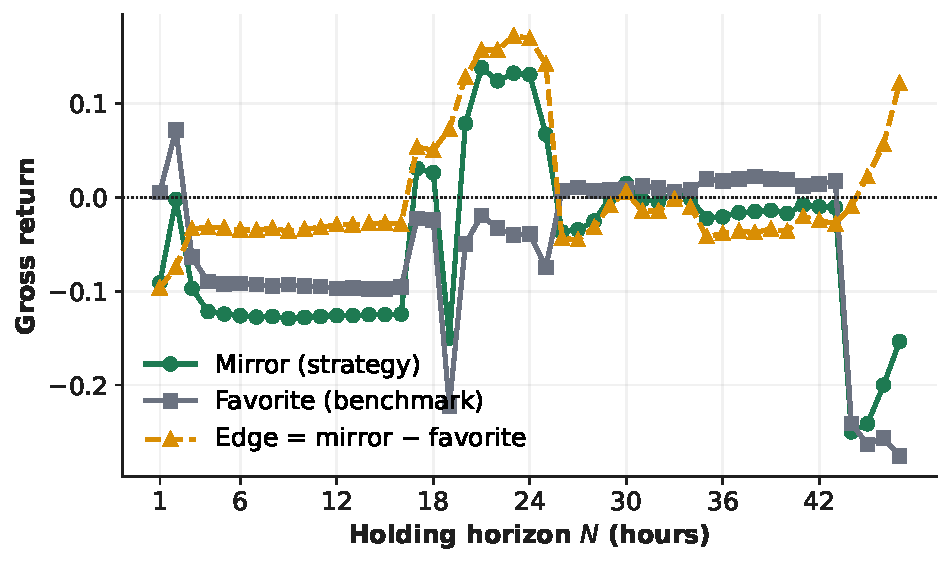
\includegraphics[width=\linewidth]{fig_edge_curve.pdf}
  \caption{Both legs and the edge.}\label{fig:edge:a}
\end{subfigure}\hfill
\begin{subfigure}{0.49\textwidth}
  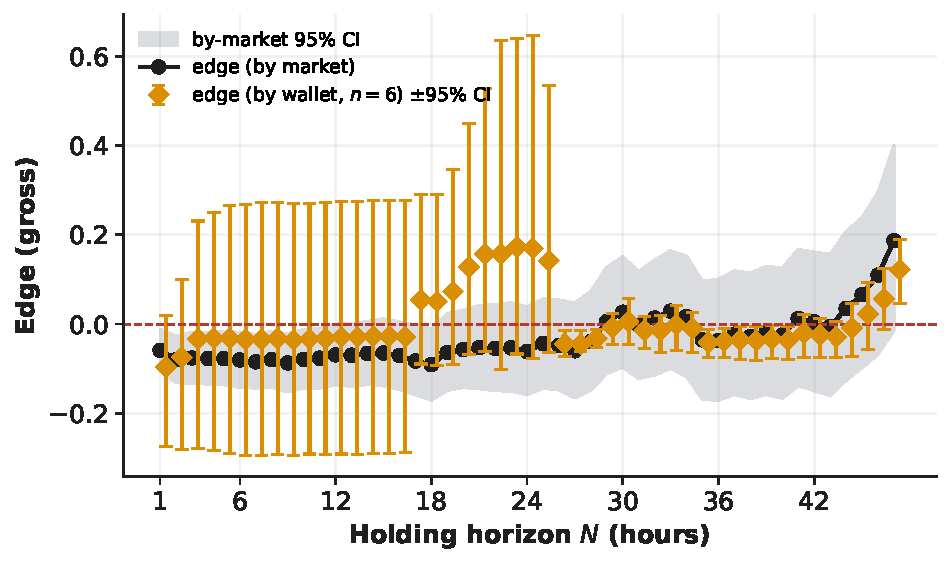
\includegraphics[width=\linewidth]{fig_edge_ci.pdf}
  \caption{Edge with bootstrap CIs.}\label{fig:edge:b}
\end{subfigure}
\caption{Forward edge-decay curve, gross of spread. \textbf{(a)} Both legs are negative at most
horizons (mirror $\approx-12\%$ to $-13\%$, favorite $\approx-9\%$ to $-10\%$ over $4$--$16$\,h;
resolution-dominated live-sports markets), with the mirror \emph{below} the favorite throughout
the short horizons. \textbf{(b)} The by-market $95\%$ bootstrap CI (shaded) excludes zero, on
the negative side, at every horizon $1$--$12$\,h, while the wide by-wallet error bars ($n{=}6$)
straddle zero there because the six wallets disagree in sign.}
\label{fig:edge}
\end{figure}

\begin{figure}[h]
\centering
\begin{subfigure}{0.49\textwidth}
  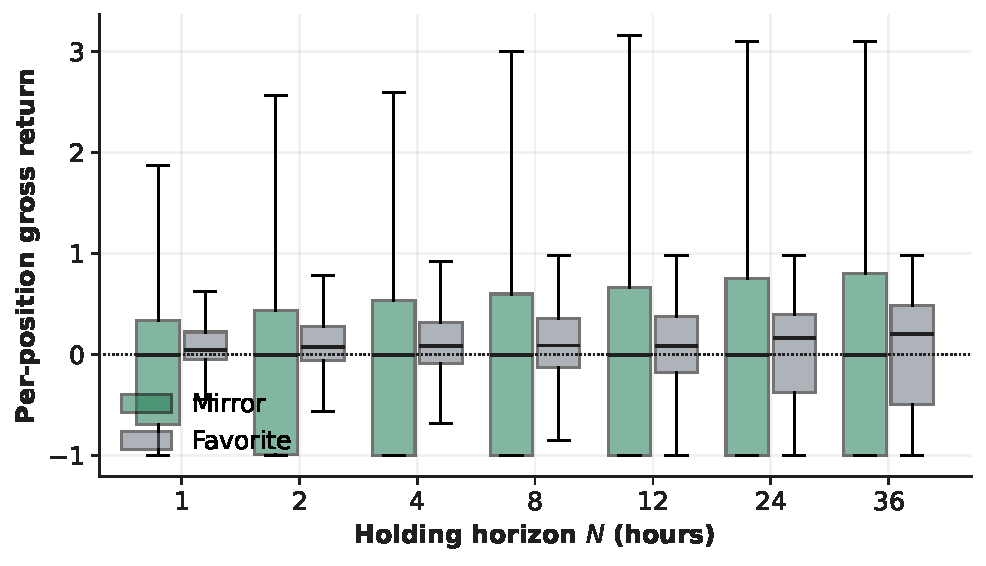
\includegraphics[width=\linewidth]{fig_return_box.pdf}
  \caption{Per-position return distributions by horizon.}
\end{subfigure}\hfill
\begin{subfigure}{0.49\textwidth}
  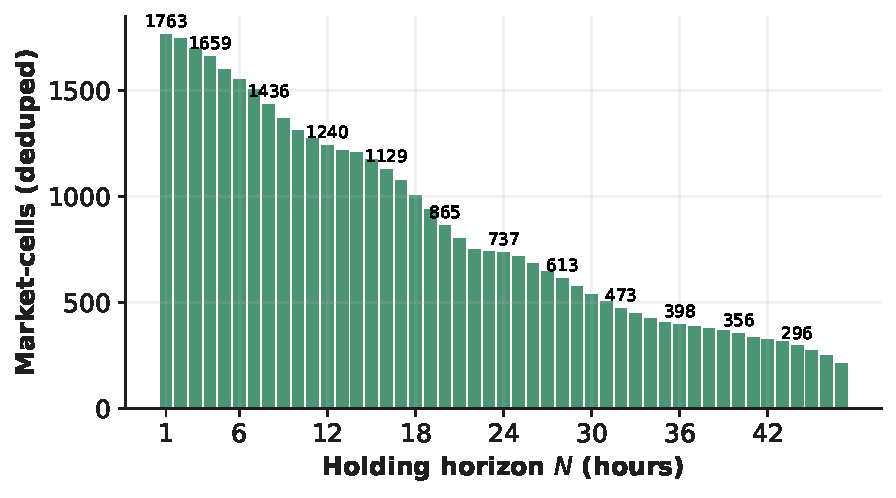
\includegraphics[width=\linewidth]{fig_sample_size.pdf}
  \caption{Deduped market-cells per horizon.}
\end{subfigure}
\caption{Forward returns and sample. \textbf{(a)} Mirror (green) and favorite (grey) per-position
gross returns; both spread widely and shift sharply negative once horizons become
resolution-dominated. \textbf{(b)} The deduped sample shrinks from $1{,}763$ market-cells at
$1$\,h to $214$ at $47$\,h; only the earliest cohort reaches the long horizons, which is the
source of the unstable long-horizon estimates.}
\label{fig:fwd2}
\end{figure}

\begin{figure}[h]
\centering
\begin{subfigure}{0.32\textwidth}
  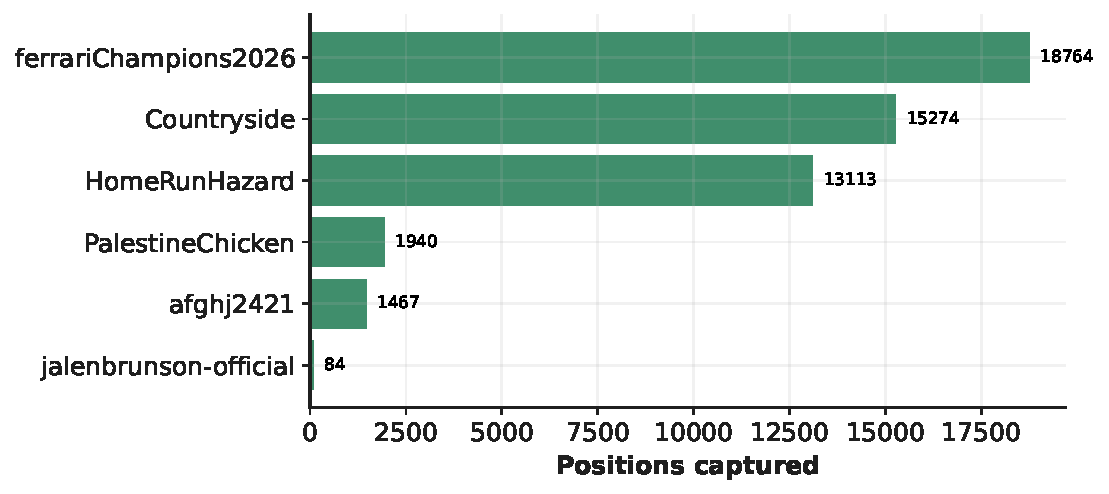
\includegraphics[width=\linewidth]{fig_wallets.pdf}
  \caption{Per-wallet activity.}
\end{subfigure}\hfill
\begin{subfigure}{0.32\textwidth}
  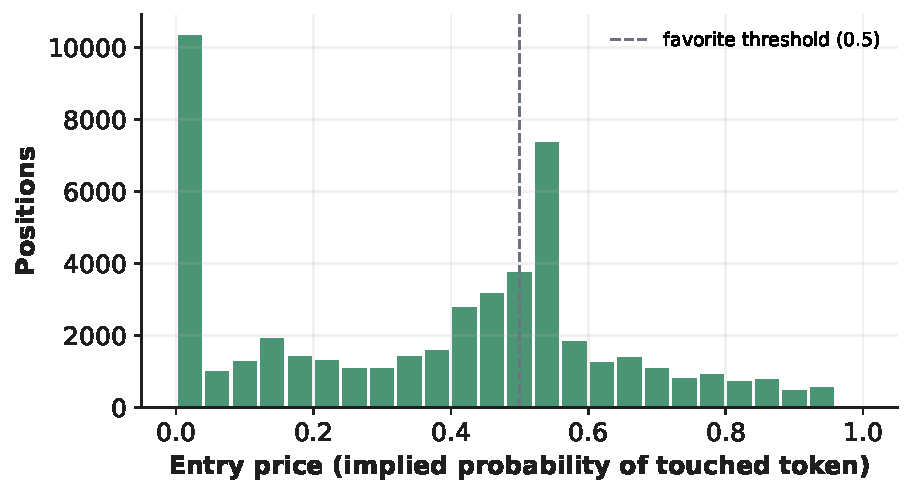
\includegraphics[width=\linewidth]{fig_entry_price.pdf}
  \caption{Entry-price distribution.}
\end{subfigure}\hfill
\begin{subfigure}{0.32\textwidth}
  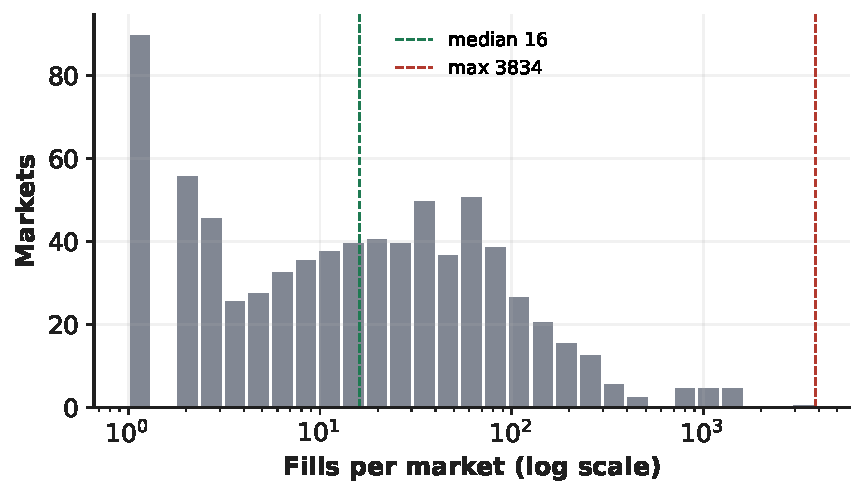
\includegraphics[width=\linewidth]{fig_fills_per_market.pdf}
  \caption{Fills per market (log).}
\end{subfigure}
\caption{Forward sample composition. \textbf{(a)} Six of ten leaderboard wallets traded; the
three largest account for $93\%$ of positions. \textbf{(b)} Entry prices span the full unit
interval (median $0.43$), a genuine mix rather than pure favorite-buying. \textbf{(c)} Fills per
market are heavy-tailed (median $16$, max $3{,}834$), which is why returns are collapsed to one
position per wallet/market/side before aggregation.}
\label{fig:fwd3}
\end{figure}

\begin{figure}[h]
\centering
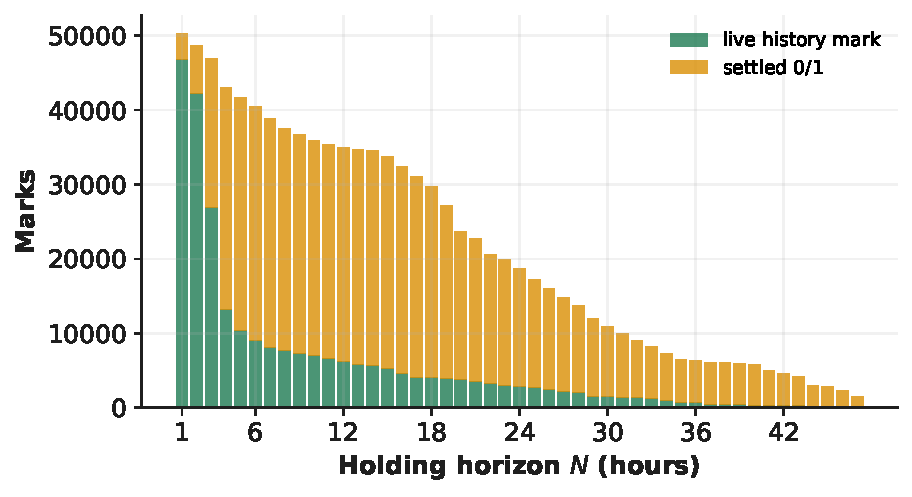
\includegraphics[width=0.66\textwidth]{fig_mark_sources.pdf}
\caption{Mark provenance by horizon: live price-history marks (green) vs.\ settled $0/1$ marks
(orange). All $999{,}012$ marks were reconstructed with none missing; longer horizons are
increasingly settlement-dominated as the short live-sports markets resolve.}
\label{fig:marks}
\end{figure}

\paragraph{(1) Clustering changes everything, now in the opposite direction.} Clustered by
\emph{market} (the correct independent unit, $n\approx214$--$1{,}763$ cells), the edge is
\emph{negative and significant} at every horizon from $1$ to $12$\,h: $-5.9\%$ to $-8.7\%$, with
the $95\%$ CI excluding zero throughout and $p$ as low as $0.003$ ($2$\,h); the band re-emerges
marginally at $17$--$18$\,h before sample attrition widens the intervals. This is the study's
first and only significant result, and it is signed \emph{against} mirroring. Clustered by
\emph{wallet} the same horizons are insignificant ($p=0.21$--$0.78$): with six clusters that
disagree in sign, the wallet-level mean is swamped by between-wallet dispersion. The interim
$12$\,h analysis had shown exactly the reverse pattern (an apparently significant by-wallet
edge against a null by-market CI), and it resolved as the small-cluster caveat predicted: the
by-wallet $p=0.006$ floor that still appears at some long horizons ($26$--$28$\,h,
$35$--$40$\,h, $47$\,h) is the minimum attainable two-sided bootstrap $p$ when all clusters
share a sign, a property of $n{=}4$ clusters rather than evidence. We caution, finally, that
the $47$ horizon tests are highly correlated (the same positions appear at every horizon they
survive to), so the $1$--$12$\,h block should be read as \emph{one} consistent finding, not
twelve independent ones.

\paragraph{(2) Small-window edges were mirages.} The extension itself is the cleanest
demonstration: at the $12$\,h interim the $1$\,h edge stood at $+2.0\%$ (by wallet, $p=0.006$);
with $8.7\times$ the sample the same horizon reads $-9.6\%$ by wallet and $-5.9\%$ by market.
Beyond ${\sim}13$\,h the estimates swing in sign with cohort composition ($+17.2\%$ by wallet
vs.\ $-5.3\%$ by market at $23$\,h) and lose significance under both clusterings; the deduped
sample attrits from $1{,}763$ cells at $1$\,h to $214$ at $47$\,h, so the long horizons are
populated only by the earliest cohort. A signal that flips sign as sample composition changes
is noise, not structure.

\paragraph{(3) Both legs lose money; the mirror loses more.} At horizons $4$--$16$\,h the
mirror returns $\approx-12\%$ to $-13\%$ and the favorite $\approx-9\%$ to $-10\%$ \emph{gross}.
The experiment never identifies a profitable strategy; the mirror now \emph{loses more} than
mechanically buying the favorite at every short horizon. That pattern is what adverse selection
on timing predicts: by the time a leader's trade is observable, the price has already moved,
and the copier systematically pays the post-information price. The deep negatives reflect the
dominance of in-game live-sports markets resolving to $0/1$ within the window: buying
\emph{either} side at volatile mid-game prices was, on average, a loser over these horizons.
All figures are \textbf{before} the modeled bid--ask spread (R6), which would subtract a
round-trip cost from \emph{both} legs and could only deepen, never reverse, the mirror's
under-performance.

% ---------------------------------------------------------------------
\section{Discussion}
% ---------------------------------------------------------------------
The two studies triangulate to the same answer from independent directions. Study~1 asks, with
full rigor and a large sample, whether \emph{any} wallet demonstrates calibration skill beyond
the market price; the answer is an unambiguous no. Study~2 asks, with a relaxed, practical
selection rule, whether naively copying current winners pays in real time; the answer is that
it reliably does \emph{not}: over $1$--$12$\,h the mirror significantly under-performs even an
also-losing favorite benchmark, gross of costs.

This convergence is the substantive result: \emph{evidence consistent with short-horizon
efficiency}. By the time a trade is observable, its information is already in the price (and
the copier, arriving after the move, pays it), so neither selecting on past calibration nor
copying current winners yields a robust edge. We state the asymmetry explicitly: an edge
$\le 0$ is consistent with efficiency but does \emph{not prove} it; the copy rule may be weak,
the window short, or the pool too small. We do not claim
to have proven these markets efficient; we claim to have \emph{failed to reject} efficiency under
two reasonable strategies, which is a meaningful negative result.

% ---------------------------------------------------------------------
\section{Limitations}
% ---------------------------------------------------------------------
\begin{itemize}\itemsep2pt
\item \textbf{R7: Wallet $\neq$ person.} Mirrored wallets may be bots, market-makers, or
copy-traders; ``skill'' is a property of an address, not an identity.
\item \textbf{Study 2 selection (R2 deviation).} Leaderboard/PnL selection is exploratory and
survivorship-prone (today's leaderboard is conditioned on having recently won).
\item \textbf{Small effective $N$.} Study~2 rests on $6$ active wallets (of $10$) over a single
window, three of them supplying $93\%$ of positions; by-wallet CIs are not trustworthy and the
inference carries on the market-cell clustering.
\item \textbf{Short, non-representative window.} $48$\,h is one two-day slice dominated by
same-day live sports; results may not generalize to politics, crypto, or longer horizons.
\item \textbf{Gross of spread.} No headline number includes transaction costs; costs can only
hurt the long mirror leg. The R6 modeled-spread sweep is the natural next step.
\item \textbf{SELL ambiguity.} Copying SELLs as opening shorts conflates fresh views with
profit-taking ($697/50{,}642$ positions, ${\sim}1.4\%$, so minor here).
\item \textbf{Mark granularity.} Marks use the at-or-before price-history point; within-minute
timing is unresolved. The favorite is fixed from the entry-time mid, never the realized winner
(R4).
\item \textbf{Modeled, not observed, depth.} There is no free historical order-book depth; the
spread is a parametric assumption throughout (R6).
\end{itemize}

% ---------------------------------------------------------------------
\section{Conclusion}
% ---------------------------------------------------------------------
Across a rigorous historical luck filter ($151$ wallets, \textbf{zero} survivors) and a live
forward mirror experiment ($50{,}642$ trades; a gross edge of $-5.9\%$ to $-8.7\%$ over
$1$--$12$\,h that is significantly \emph{negative} under the correct market-level clustering,
$p\le0.05$ at every such horizon), \textbf{we find no exploitable mirror-trading edge over a
buy-the-favorite benchmark on Polymarket at short horizons; if anything, mirroring reliably
pays the post-information price.} The most defensible reading is that these markets price
observable trading information efficiently enough that neither past-calibration selection nor
copy-the-winner selection beats the favorite after honest accounting; the significant
short-horizon under-performance is exactly what adverse price impact predicts. This is a clean
negative result and, by the standard set at the outset, a successful one.

% ---------------------------------------------------------------------
\appendix
\section{Reproducibility}
\textbf{Single source of truth:} \texttt{config.py} (windows, floors,
$n_{\text{bootstrap}}=10{,}000$, \texttt{seed}=20260602, spread presets); every stochastic step
takes the seed explicitly. \textbf{Study 1:} \texttt{notes/\_discover.py},
\texttt{notes/\_luckfilter.py}, \texttt{notes/\_diag.py} over cached Gamma/Data pulls; scorer and
null in \texttt{polymirror/scorer.py} and \texttt{polymirror/stats.py}. \textbf{Study 2:}
watchlist via \texttt{notes/\_leaderboard\_watchlist.py}; on-demand puller \texttt{forward\_pull.py}
(state in \texttt{data/forward/experiment.json}, keyed by transaction hash, idempotent); API
helpers \texttt{get\_activity}, \texttt{get\_price\_history}, \texttt{get\_clob\_midpoint},
\texttt{get\_market\_gamma(fresh=)} in \texttt{polymirror/polyapi.py}. \textbf{Outputs}
(\texttt{data/forward/}): \texttt{positions.csv}, \texttt{marks\_long.csv} (one row per trade
$\times$ horizon, with strat/bench/edge), \texttt{edge\_curve.csv}, \texttt{edge\_curve\_final.csv}
(edge with bootstrap CIs under both clusterings). \textbf{Inference:} \texttt{bootstrap\_mean\_ci},
\texttt{bootstrap\_two\_sided\_p}, and \texttt{benjamini\_hochberg} in \texttt{polymirror/stats.py},
all seeded.

\section{Key parameters}
\begin{table}[h]
\centering
\small
\begin{tabular}{@{}ll@{}}
\toprule
Train / test split & 2025-01-01 $\to$ 2025-09-01 $\to$ 2026-01-01 (R1) \\
Accuracy metric & Brier (log loss available) \\
Activity floors & $\{8,10,15\}$ positions per wallet \\
Luck null & $y_i^\ast\sim\mathrm{Bernoulli}(p_i)$, $10{,}000$ draws, BH-FDR, $\alpha=0.05$ \\
Forward window & 2026-06-07 20:04 $\to$ 2026-06-09 20:04 UTC \\
Forward horizons & $N\in\{1,2,\dots,48\}$ hours ($N{=}48$ empty: it falls exactly on the window cap) \\
Spread presets (R6) & optimistic 1.0\textcent\ / base 2.5\textcent\ / conservative 5.0\textcent\ (full spread at mid) \\
Seed & 20260602 \\
\bottomrule
\end{tabular}
\end{table}

\section{Full forward edge-decay table}\label{app:fulledge}
Table~\ref{tab:edgefull} reports the complete edge-decay curve at every populated horizon,
under both clusterings, from \texttt{data/forward/edge\_curve\_final.csv}.

\begin{table}[p]
\centering
\caption{Complete forward edge-decay curve, all $47$ populated horizons (gross of spread; one
position per wallet/market/side). $n_w$ is the number of wallet clusters and ``cells'' the
number of independent market-cells; columns otherwise as in Table~\ref{tab:edge}. $95\%$ CIs
and two-sided $p$-values are from the seeded $10{,}000$-resample bootstrap. The horizon tests
are highly correlated across rows (overlapping positions) and should not be read as
independent.}
\label{tab:edgefull}
\scriptsize
\setlength{\tabcolsep}{3pt}
\begin{tabular}{@{}rrr rr rcc rcc@{}}
\toprule
& & & \multicolumn{2}{c}{Returns (gross)} & \multicolumn{3}{c}{By wallet} & \multicolumn{3}{c}{By market} \\
\cmidrule(lr){4-5}\cmidrule(lr){6-8}\cmidrule(lr){9-11}
$N$(h) & $n_w$ & cells & Mirror & Favorite & Edge & 95\% CI & $p$ & Edge & 95\% CI & $p$ \\
\midrule
1 & 6 & 1{,}763 & $-0.091$ & $+0.005$ & $-0.096$ & $[-0.274,+0.019]$ & 0.213 & $-0.059$ & $[-0.105,-0.012]$ & 0.013 \\
2 & 6 & 1{,}744 & $-0.002$ & $+0.072$ & $-0.074$ & $[-0.281,+0.100]$ & 0.448 & $-0.080$ & $[-0.132,-0.026]$ & 0.003 \\
3 & 6 & 1{,}696 & $-0.097$ & $-0.064$ & $-0.033$ & $[-0.279,+0.231]$ & 0.714 & $-0.076$ & $[-0.133,-0.019]$ & 0.011 \\
4 & 6 & 1{,}659 & $-0.122$ & $-0.090$ & $-0.032$ & $[-0.283,+0.249]$ & 0.735 & $-0.077$ & $[-0.135,-0.020]$ & 0.010 \\
5 & 6 & 1{,}597 & $-0.124$ & $-0.092$ & $-0.032$ & $[-0.290,+0.265]$ & 0.753 & $-0.078$ & $[-0.136,-0.016]$ & 0.014 \\
6 & 6 & 1{,}550 & $-0.126$ & $-0.092$ & $-0.035$ & $[-0.295,+0.269]$ & 0.759 & $-0.081$ & $[-0.142,-0.019]$ & 0.011 \\
7 & 6 & 1{,}506 & $-0.128$ & $-0.093$ & $-0.035$ & $[-0.295,+0.272]$ & 0.760 & $-0.085$ & $[-0.144,-0.023]$ & 0.007 \\
8 & 6 & 1{,}436 & $-0.127$ & $-0.094$ & $-0.033$ & $[-0.293,+0.272]$ & 0.767 & $-0.080$ & $[-0.142,-0.016]$ & 0.015 \\
9 & 6 & 1{,}368 & $-0.129$ & $-0.093$ & $-0.036$ & $[-0.294,+0.269]$ & 0.766 & $-0.087$ & $[-0.152,-0.022]$ & 0.009 \\
10 & 6 & 1{,}310 & $-0.128$ & $-0.094$ & $-0.034$ & $[-0.291,+0.270]$ & 0.767 & $-0.079$ & $[-0.144,-0.012]$ & 0.020 \\
11 & 6 & 1{,}274 & $-0.127$ & $-0.095$ & $-0.032$ & $[-0.293,+0.273]$ & 0.767 & $-0.077$ & $[-0.144,-0.010]$ & 0.025 \\
12 & 6 & 1{,}240 & $-0.126$ & $-0.097$ & $-0.029$ & $[-0.291,+0.275]$ & 0.776 & $-0.069$ & $[-0.136,-0.000]$ & 0.050 \\
13 & 6 & 1{,}218 & $-0.126$ & $-0.097$ & $-0.029$ & $[-0.292,+0.275]$ & 0.776 & $-0.070$ & $[-0.140,+0.001]$ & 0.054 \\
14 & 6 & 1{,}209 & $-0.125$ & $-0.098$ & $-0.027$ & $[-0.289,+0.276]$ & 0.776 & $-0.066$ & $[-0.136,+0.006]$ & 0.071 \\
15 & 6 & 1{,}177 & $-0.125$ & $-0.098$ & $-0.027$ & $[-0.289,+0.276]$ & 0.776 & $-0.065$ & $[-0.138,+0.012]$ & 0.089 \\
16 & 6 & 1{,}129 & $-0.124$ & $-0.096$ & $-0.029$ & $[-0.288,+0.276]$ & 0.776 & $-0.071$ & $[-0.147,+0.005]$ & 0.067 \\
17 & 6 & 1{,}074 & $+0.031$ & $-0.023$ & $+0.054$ & $[-0.090,+0.290]$ & 0.673 & $-0.083$ & $[-0.159,-0.002]$ & 0.047 \\
18 & 6 & 1{,}007 & $+0.026$ & $-0.024$ & $+0.051$ & $[-0.094,+0.290]$ & 0.673 & $-0.091$ & $[-0.171,-0.011]$ & 0.026 \\
19 & 5 & 940 & $-0.150$ & $-0.223$ & $+0.073$ & $[-0.091,+0.347]$ & 0.656 & $-0.064$ & $[-0.149,+0.024]$ & 0.148 \\
20 & 4 & 865 & $+0.079$ & $-0.049$ & $+0.128$ & $[-0.068,+0.450]$ & 0.552 & $-0.057$ & $[-0.142,+0.031]$ & 0.204 \\
21 & 4 & 805 & $+0.138$ & $-0.019$ & $+0.157$ & $[-0.062,+0.528]$ & 0.552 & $-0.053$ & $[-0.145,+0.042]$ & 0.265 \\
22 & 4 & 751 & $+0.124$ & $-0.033$ & $+0.157$ & $[-0.102,+0.635]$ & 0.626 & $-0.055$ & $[-0.149,+0.044]$ & 0.262 \\
23 & 4 & 743 & $+0.133$ & $-0.040$ & $+0.172$ & $[-0.067,+0.639]$ & 0.626 & $-0.053$ & $[-0.151,+0.048]$ & 0.280 \\
24 & 4 & 737 & $+0.131$ & $-0.039$ & $+0.170$ & $[-0.078,+0.646]$ & 0.626 & $-0.062$ & $[-0.158,+0.038]$ & 0.211 \\
25 & 4 & 718 & $+0.067$ & $-0.075$ & $+0.142$ & $[-0.064,+0.534]$ & 0.626 & $-0.044$ & $[-0.144,+0.056]$ & 0.382 \\
26 & 4 & 687 & $-0.037$ & $+0.007$ & $-0.044$ & $[-0.072,-0.015]$ & 0.006 & $-0.048$ & $[-0.148,+0.054]$ & 0.352 \\
27 & 4 & 645 & $-0.034$ & $+0.011$ & $-0.045$ & $[-0.061,-0.015]$ & 0.006 & $-0.060$ & $[-0.166,+0.048]$ & 0.275 \\
28 & 4 & 613 & $-0.025$ & $+0.007$ & $-0.032$ & $[-0.053,-0.011]$ & 0.006 & $-0.039$ & $[-0.149,+0.073]$ & 0.475 \\
29 & 4 & 575 & $+0.000$ & $+0.008$ & $-0.008$ & $[-0.046,+0.023]$ & 0.652 & $+0.006$ & $[-0.111,+0.128]$ & 0.929 \\
30 & 4 & 540 & $+0.015$ & $+0.009$ & $+0.006$ & $[-0.045,+0.057]$ & 0.721 & $+0.026$ & $[-0.097,+0.151]$ & 0.698 \\
31 & 4 & 505 & $-0.002$ & $+0.012$ & $-0.015$ & $[-0.055,+0.016]$ & 0.496 & $-0.003$ & $[-0.122,+0.118]$ & 0.952 \\
32 & 4 & 473 & $-0.005$ & $+0.010$ & $-0.014$ & $[-0.063,+0.019]$ & 0.648 & $+0.013$ & $[-0.115,+0.144]$ & 0.841 \\
33 & 4 & 450 & $+0.005$ & $+0.006$ & $-0.002$ & $[-0.059,+0.041]$ & 0.997 & $+0.029$ & $[-0.100,+0.164]$ & 0.666 \\
34 & 4 & 426 & $-0.002$ & $+0.008$ & $-0.010$ & $[-0.064,+0.026]$ & 0.678 & $+0.017$ & $[-0.118,+0.153]$ & 0.838 \\
35 & 4 & 407 & $-0.022$ & $+0.020$ & $-0.042$ & $[-0.076,-0.012]$ & 0.006 & $-0.035$ & $[-0.169,+0.096]$ & 0.591 \\
36 & 4 & 398 & $-0.021$ & $+0.018$ & $-0.038$ & $[-0.075,-0.009]$ & 0.006 & $-0.037$ & $[-0.171,+0.100]$ & 0.585 \\
37 & 4 & 388 & $-0.016$ & $+0.020$ & $-0.036$ & $[-0.080,-0.006]$ & 0.006 & $-0.023$ & $[-0.158,+0.119]$ & 0.735 \\
38 & 4 & 377 & $-0.015$ & $+0.022$ & $-0.037$ & $[-0.082,-0.006]$ & 0.006 & $-0.028$ & $[-0.167,+0.114]$ & 0.688 \\
39 & 4 & 368 & $-0.014$ & $+0.020$ & $-0.034$ & $[-0.078,-0.004]$ & 0.006 & $-0.017$ & $[-0.158,+0.129]$ & 0.808 \\
40 & 4 & 356 & $-0.017$ & $+0.019$ & $-0.036$ & $[-0.080,-0.006]$ & 0.006 & $-0.025$ & $[-0.167,+0.125]$ & 0.751 \\
41 & 4 & 336 & $-0.008$ & $+0.012$ & $-0.021$ & $[-0.076,+0.020]$ & 0.501 & $+0.012$ & $[-0.138,+0.168]$ & 0.873 \\
42 & 4 & 325 & $-0.010$ & $+0.014$ & $-0.024$ & $[-0.076,+0.013]$ & 0.403 & $+0.005$ & $[-0.150,+0.161]$ & 0.953 \\
43 & 4 & 316 & $-0.011$ & $+0.018$ & $-0.028$ & $[-0.076,+0.005]$ & 0.158 & $-0.006$ & $[-0.160,+0.157]$ & 0.930 \\
44 & 4 & 296 & $-0.250$ & $-0.241$ & $-0.009$ & $[-0.073,+0.047]$ & 0.742 & $+0.035$ & $[-0.127,+0.207]$ & 0.687 \\
45 & 4 & 275 & $-0.241$ & $-0.264$ & $+0.022$ & $[-0.057,+0.094]$ & 0.597 & $+0.066$ & $[-0.098,+0.239]$ & 0.447 \\
46 & 4 & 249 & $-0.200$ & $-0.257$ & $+0.056$ & $[-0.011,+0.124]$ & 0.115 & $+0.110$ & $[-0.068,+0.295]$ & 0.231 \\
47 & 4 & 214 & $-0.154$ & $-0.275$ & $+0.122$ & $[+0.046,+0.190]$ & 0.006 & $+0.187$ & $[-0.015,+0.400]$ & 0.074 \\
\bottomrule
\end{tabular}
\end{table}

\end{document}
